\documentclass{homework}
\usepackage[spanish]{babel}
% Paquetes para incluir figuras generadas por las simulaciones
\usepackage{graphicx}
\usepackage{float}
\decimalpoint

\author{José Ángel Aké}
\class{Teoría cuántica de campos y materia condensada}
\date{\today}
\title{Ejercicio extra: Simulación BdG}
\address{Posgrado en Ciencias Físicas, UNAM}
\setunitname{Pregunta}

\begin{document}  \maketitle


% Referencias
\section*{Resultados BdG (Bogoliubov--de Gennes)}
Los resultados mostrados a continuación fueron obtenidos con el solver BdG implementado en el cuaderno de simulación. Se incluyen (i) el perfil espacial del parámetro de orden $|\Delta_i|$ a temperatura $T=0$, y (ii) la curva del parámetro de orden promedio $\langle|\Delta|\rangle$ en función de la temperatura que permite estimar la temperatura crítica $T_c$.

\begin{figure}[H]
	\centering
	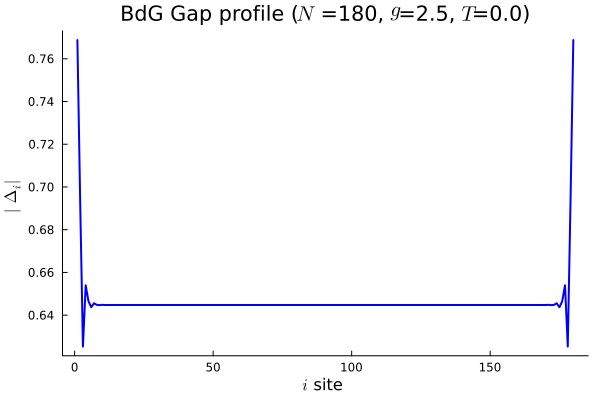
\includegraphics[width=0.49\textwidth]{../BdG_gap_profile.png}
	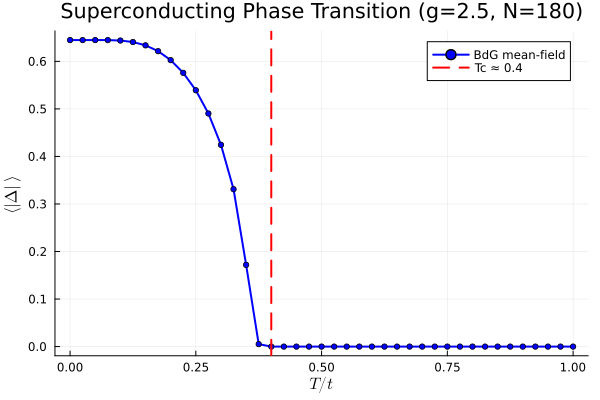
\includegraphics[width=0.49\textwidth]{../phase_transition.png}
	\caption{Izquierda: Perfil espacial del módulo del gap $|\Delta_i|$ a $T=0$ (parámetros ejemplo: $N=180$, $t=1$, $\mu=-1.0$, $g=2.5$, mezcla/ $\text{mix}=0.3$). Se aprecia que el parámetro de orden es esencialmente constante fuera de la frontera y exhibe oscilaciones cerca de las fronteras por efectos de tamaño finito. 
	Derecha: Promedio $\langle|\Delta|\rangle$ vs temperatura (mismos parámetros usados que en la figura izquierda). La intersección con el umbral elegido ($\sim10^{-3}$) da una estimación de $T_c$ (en este caso $T_c\approx0.1$ en unidades de $t$ según el barrido numérico mostrado).}
	\label{fig:bdg_results}
\end{figure}

Notar que: El acoplamiento $g$ controla la magnitud del gap en $T=0$ y la temperatura crítica. En la figura de la izquierda se usó una condición inicial pequeña con ruido y la mezcla (``mix'') en el algoritmo iterativo se ajustó para favorecer la convergencia estable.

% Referencias
%\bibliographystyle{plain}
%\bibliography{citations}

\end{document}

